% !TEX TS-program = pdflatex
\documentclass{aa}

% ---------- Layout ----------
% geometry and setspace not needed with aa.cls

% ---------- Math / Tables / Figures ----------
\usepackage{amsmath, amssymb}
\usepackage{graphicx}
\usepackage{booktabs}
\usepackage{siunitx}
\usepackage{pgfplotstable}
\pgfplotsset{compat=1.15}

% ---------- References / Links ----------
% natbib loaded by aa.cls
\usepackage[hidelinks]{hyperref}

% ---------- Convenience ----------
% \usepackage{microtype}

% ---------- Title metadata ----------
\title{Diagnosing sky-structured parallax residuals in Gaia DR3 via concentration and leverage tests on a quasar reference sample}
\author{M. Blumhardt\inst{1}}
\institute{Independent Researcher}
\date{}
\titlerunning{Concentration and leverage diagnostics for Gaia DR3 parallax residuals}
\authorrunning{M. Blumhardt}

\begin{document}
\abstract{A reproducible diagnostic workflow characterizes sky-structured parallax residuals in Gaia DR3 using quasars as an approximate zero-parallax reference population. The QSO parallax field functions as a reference-frame residual surface whose spatial topology may reflect calibration structure, contamination, or other unmodeled effects. These diagnostics complement existing approaches that characterize mean parallax bias or angular covariance by instead quantifying whether the residual field is dominated by a small fraction of sky regions or reflects broadly distributed calibration structure. Metrics quantify that topology along two orthogonal axes: (i) concentration of weighted contribution across the sky via a Lorenz-style curve and Top-20\% contribution statistic, and (ii) leverage of extreme sky regions via a diagnostic top-$K$ masking stress test. Locked dataset snapshot, fixed quality cuts, and pre-specified statistics yield a moderately concentrated but scale-persistent field (Top-20\% contribution $\approx 0.60$ across NSIDE 4--32, exceeding footprint-only null of $\approx 0.34$) with low leverage to small-$K$ masking. Diagnostics quantify spatial behavior under aggregation and masking without identifying physical origin.}

\keywords{astrometry -- parallaxes -- methods: statistical -- quasars: general}

\maketitle

% --- BEGIN sections/introduction.tex ---
\section{Introduction}

Gaia parallaxes serve as foundational inputs to a broad range of astrophysical and cosmological analyses. Residual calibration and observation-geometry effects imprint coherent, sky-structured patterns in inferred parallaxes. Undiagnosed patterns risk propagation into downstream inference and may be misinterpreted as physical sky signals.

Quasars (QSOs) serve as an effectively zero-parallax reference population. The resulting parallax field constitutes a reference-frame residual surface whose spatial topology may reflect calibration residuals, contamination, or other unmodeled effects. The objective is characterization of that topology with emphasis on operational consequences for downstream use. Three conceptually separate axes are distinguished: (i) field amplitude (magnitude of sky-structured variation), (ii) concentration (fraction of weighted contribution carried by a minority of sky regions), and (iii) leverage (sensitivity of amplitude to exclusion of a small number of extreme regions).

This work is intended to complement, rather than replace, existing approaches to characterizing Gaia parallax systematics. Whereas prior studies primarily focus on estimating the magnitude of parallax bias or modeling its spatial correlation structure, the goal here is to provide diagnostic statistics that classify what kind of sky-structured systematic is present. These diagnostics answer a mitigation question distinct from bias estimation and covariance modeling: whether systematic structure is hotspot-dominated and therefore plausibly maskable, or distributed across the footprint and therefore requiring explicit systematic modeling in downstream analyses.

A minimal, locked set of statistics and quality cuts is defined prior to inspection of results. The approach centers the contribution on diagnostic tooling rather than post-hoc rationalization.

The workflow quantifies whether a residual field appears (a) outlier-dominated or (b) broadly distributed via concentration and leverage. Validation of QSOs as an astrophysical zero-parallax frame is not performed. Mechanism identification (scan law, chromaticity, contamination, etc.) is not performed. Classification of calibration versus astrophysics is not performed.

\subsection{Prior work on quasar-based parallax diagnostics}

Quasars provide an effectively zero-parallax reference population and have therefore played a central role in the diagnosis and validation of Gaia parallax systematics across recent data releases. Existing work using quasars as diagnostics can be broadly grouped into three methodological classes: parametric parallax-bias modeling, spatial mapping of quasar parallax residuals, and characterization of angular covariance or correlation structure.

The canonical treatment of parallax bias in Gaia EDR3 and DR3 is provided by Lindegren et al.\ (2021b), who use quasar parallaxes to model the systematic offset as a function of magnitude, colour proxy, and sky position, yielding correction recipes ($Z_5$, $Z_6$) that are now widely applied in downstream analyses. This correction-oriented framework is designed to estimate and remove an expected bias field rather than to classify the topology of residual sky structure.

Independent analyses have also examined the spatial structure of quasar parallax residuals through explicit sky mapping. Groenewegen (2021), for example, presents HEALPix-resolved maps at multiple angular resolutions and demonstrates that spatially coherent residuals persist even after applying global corrections. Such approaches provide intuitive visualization and regional summaries of parallax systematics but typically do not quantify whether the total residual signal is dominated by a small subset of sky regions or distributed broadly across the footprint.

A complementary line of work characterizes parallax systematics through angular covariance or correlation analyses. Using quasars to anchor large angular scales, often in combination with other reference populations, these studies quantify correlation lengths and systematic floors in Gaia parallaxes (e.g.\ Ma\'iz Apell\'aniz et al.\ 2021). Zinn (2021) extends this covariance-based validation to brighter magnitudes and smaller angular scales using asteroseismic parallaxes. While such analyses characterize how parallax errors correlate as a function of separation, they do not directly address questions of concentration or leverage of the residual field.

The present work is complementary to all three approaches. Rather than proposing a new correction model, constructing alternative sky maps, or estimating an angular covariance function, this work introduces diagnostic statistics quantifying the concentration of weighted parallax residual contribution across the sky and the leverage of extreme regions on global summary measures. These diagnostics are designed to answer a distinct operational question: whether sky-structured residuals are dominated by a small number of maskable regions or instead reflect a distributed calibration mode that affects most of the sky.

% --- END sections/introduction.tex ---
% --- BEGIN sections/methods.tex ---
\section{Methods}

All statistics are pre-specified before inspection of results; no metrics were added post hoc, and all pre-specified statistics are reported.
Pre-specified diagnostics were:
\begin{itemize}
\item $S$ (NSIDE=32)
\item $C_{0.20}$ at NSIDE 4, 8, 16, 32
\item Top-$K$ masking for $K=\{5,10,20\}$
\item Permutation-null $C_{0.20}$
\end{itemize}
No other metrics were computed.

\subsection{Data snapshot and fields}
Analyses utilize a single frozen ``analysis-ready'' Parquet dataset containing Gaia DR3 source identifiers, sky coordinates (RA/Dec), parallax, and standard Gaia quality/coverage proxies. The pipeline design prioritizes reproducibility: data snapshot, cuts, and statistics remain locked before inspection of outcomes.

\subsection{Quality cuts (locked)}
Minimal quality cuts remove grossly unstable astrometric solutions while preserving large-scale sky footprint: (i) non-missing values required for RA, Dec, parallax, RUWE, and visibility periods used; (ii) sources retained with visibility\_periods\_used $\ge 8$; (iii) sources retained with RUWE $\le 1.4$. No additional thresholds are introduced after inspection.

\subsection{HEALPix binning and per-pixel statistic}
Sky discretization employs HEALPix in RING ordering. The primary map and global spatial summary use NSIDE = 32. Each occupied pixel $p$ receives per-pixel median parallax computation:
\[
\tilde{\varpi}_{p} = \mathrm{median}\{\varpi_i : i \in p\}.
\]
Median aggregation reduces sensitivity to outliers while preserving coherent sky structure.

NSIDE=32 (~1.8° pixels) captures large-scale scanning-law footprint while maintaining sufficient source counts per pixel for robust median estimation. This resolution is appropriate for characterizing the scale of dominant residual structure affecting global reference-frame behavior; finer-scale analysis would require different diagnostic frameworks optimized for high-frequency patterns.

\subsection{\texorpdfstring{Global amplitude statistic $S$}{Global amplitude statistic S} }
Amplitude of sky-structured parallax variation receives summary via
\[
S = \mathrm{SD}\left(\{\tilde{\varpi}_{p}\}\right),
\]
the sample standard deviation (ddof=1) of per-pixel median parallaxes across occupied NSIDE=32 pixels.

Uncertainty quantification employs a bootstrap over pixels: pixels are resampled with replacement (1000 resamples) and $S$ recomputed for each resample. The 95\% interval corresponds to the 2.5\% and 97.5\% quantiles of the bootstrap distribution. The bootstrap targets uncertainty in dispersion of the spatial field rather than within-pixel median estimation. Pixel-bootstrap intervals constitute a heuristic uncertainty summary; spatial correlations may reduce effective degrees of freedom.

\subsection{\texorpdfstring{Concentration diagnostic: Lorenz curve and Top-20\% contribution}{Concentration diagnostic: Lorenz curve and Top-20 percent contribution}}
Quantification of whether field magnitude is carried by a minority of sky regions employs a nonnegative contribution weight at a chosen HEALPix superpixel resolution:
\[
w_s = N_s \, |\tilde{\varpi}_s|,
\]
where $N_s$ denotes the number of sources in superpixel $s$ and $\tilde{\varpi}_s$ denotes the median parallax within $s$. A Lorenz-style cumulative contribution curve is computed by sorting superpixels by $w_s$ in descending order and plotting cumulative fraction of $\sum_s w_s$ versus cumulative fraction of superpixels.

Concentration is summarized via the Top-20\% contribution statistic
\[
C_{0.20} = \frac{\sum_{s \in \text{top 20\%}} w_s}{\sum_s w_s},
\]
where ``top 20\%'' refers to the top $\lceil 0.2 n \rceil$ occupied superpixels by $w_s$. $C_{0.20}$ is reported at NSIDE=32 with assessment of stability across NSIDE $\in \{4,8,16,32\}$. The Top-20\% threshold follows conventional Pareto-style concentration summaries and functions as a fixed reporting convention rather than a tuned parameter; sensitivity to angular resolution is assessed separately via the NSIDE stability analysis. Absolute value $|\tilde{\varpi}_s|$ quantifies heterogeneity magnitude irrespective of sign.

A sensitivity check employs an unweighted variant $C_{0.20}(|\cdot|)$ with $w_s = |\tilde{\varpi}_s|$ (dropping $N_s$) to assess whether the descriptive pattern changes with removal of density weighting.

\subsection{\texorpdfstring{Leverage diagnostic: top-\texorpdfstring{$K$}{K} masking stress test}{Leverage diagnostic: top-K masking stress test} (not corrective)}
A diagnostic stress test probes whether global amplitude $S$ is driven by a small number of extreme regions: sources in top-ranked NSIDE=8 superpixels are excluded according to a precomputed regional contribution ranking and $S$ recomputed at NSIDE=32 on the masked dataset. The ranking functions as an independent leverage probe; masking does not serve a corrective procedure.

Results are reported for $K \in \{5,10,20\}$ as the primary stress test set. These values span the regime in which region exclusion remains operationally inexpensive ($\lesssim 4\%$ of sky); the set probes fragility to small-area excision rather than optimizing a masking strategy. Masking definition on a coarser partition tests whether large-area regions dominate NSIDE=32 dispersion.

\subsection{Permutation null for footprint-driven concentration}
Assessment of whether observed concentration reflects spatial clustering of parallax residuals rather than heterogeneous sky footprint and source density employs a permutation null: per-superpixel median parallaxes $\tilde{\varpi}_s$ are randomly permuted across superpixels while $N_s$ and sky positions remain fixed. The null distribution of $C_{0.20}$ is estimated from 1000 permutations at NSIDE=32. The same procedure is applied to the unweighted variant $w_s = |\tilde{\varpi}_s|$ as a density-removal sensitivity check.

% --- END sections/methods.tex ---
% --- BEGIN sections/results.tex ---
\section{Results}

\subsection{Sky-structured parallax field and concentration diagnostics}
Figure~1 displays the NSIDE=32 sky map of per-pixel median parallax and the corresponding Lorenz-style cumulative contribution curve constructed from $w_s = N_s |\tilde{\varpi}_s|$ at NSIDE=32. The Top-20\% contribution statistic remains stable across angular resolutions NSIDE 4--32, with $C_{0.20}$ ranging approximately 0.60--0.64. A moderately concentrated but scale-persistent sky-structured field results: variation is neither uniform ($C_{0.20} \approx 0.20$ expected) nor dominated by a small number of extreme regions ($C_{0.20} \rightarrow 1$). Stability of $C_{0.20}$ across two orders of magnitude in angular resolution disfavors confinement of the structure to a narrow angular scale.

\paragraph{Comparison to existing spatial diagnostics.}
The reported concentration values ($C_{0.20} \approx 0.60$--0.64 across NSIDE = 4--32) quantify an aspect of spatial structure that is not captured by commonly used diagnostics. Spatial mapping approaches, such as HEALPix-resolved mean parallax maps (e.g.\ Groenewegen 2021), reveal the presence and approximate amplitude of regional variations but do not quantify the inequality of contribution across regions. Angular covariance analyses (e.g.\ Lindegren et al.\ 2021a; Ma\'iz Apell\'aniz et al.\ 2021) characterize correlation length and coherence scale but do not directly quantify whether the field is dominated by a small number of regions or broadly distributed. A uniformly distributed field would yield $C_{0.20} \approx 0.20$, while a footprint-only null produces $C_{0.20} \approx 0.34$. The observed values indicate that approximately 20\% of sky regions account for ${\sim}60\%$ of the weighted signal, placing the Gaia DR3 quasar parallax field in a regime of moderate but distributed concentration rather than hotspot-dominated structure.

\paragraph{Null test for footprint-driven concentration.}
Assessment of whether observed concentration reflects spatial clustering of parallax residuals rather than heterogeneous sky footprint and source density employs a permutation null: per-superpixel median parallaxes $\tilde{\varpi}_s$ receive random permutation across superpixels while $N_s$ and sky positions remain fixed. Across 1000 permutations at NSIDE=32, the shuffled field yields $C_{0.20}$ with median 0.34 and 95\% interval [0.31, 0.37], substantially below observed $\approx 0.60$. Repetition with $w_s = |\tilde{\varpi}_s|$ (density weighting dropped) yields similar results: observed $C_{0.20} \approx 0.58$--0.62 while shuffled null remains $\approx 0.33$. Detected concentration exceeds the null expectation from footprint geometry alone, indicating spatial clustering in the parallax residual field.

\subsection{Leverage diagnostics via top-\texorpdfstring{$K$}{K} masking}
A diagnostic stress test excludes sources in top-ranked NSIDE=8 superpixels and recomputes global amplitude statistic $S$ at NSIDE=32. For $K \le 20$, removal of the most extreme regions produces negligible change in $S$; substantial reductions occur only after excision of many regions (Table~2).

Low leverage with respect to the most extreme regions under this masking scheme results: global amplitude is not controlled by a small set of hotspots. Field amplitude reflects contributions from a broad fraction of sky. The ranking used for masking derives from an independently computed regional contribution estimator at NSIDE=8. Top-$K$ results are interpreted strictly as a leverage diagnostic rather than continuation of Lorenz-style concentration analysis.

The test probes dominance of a few large sky patches (NSIDE=8 resolution) on the statistic. The test does not address whether fine-scale masking (higher NSIDE) alters the field or serves as a mitigation strategy.

\subsection{Observation-history proxy correlation}

To test whether spatial concentration correlates with Gaia's observation geometry, median observation-history proxies were computed for each NSIDE=16 superpixel and distributions compared between all regions and top-20\% contributors (ranked by $w_s$) (Figure 3).

Top-contributing regions are statistical outliers in all four proxies (Mann--Whitney $U$ test, all $p < 0.001$). This strong association with observation-history proxies is consistent with, though not uniquely diagnostic of, survey-geometry--coupled systematics.

\subsection{Joint interpretation: topology and fragility}
Concentration and leverage diagnostics characterize the observed QSO parallax field as moderately concentrated, scale-persistent, and low top-$K$ leverage. Moderate inequality in weighted contribution, stability across angular resolutions, and weak sensitivity to removal of a small number of extreme regions occur. Field variance appears broadly distributed rather than hotspot-dominated.




These proxies reflect observation-history and data-quality covariates consistent with calibration systematics. They do not uniquely identify a single mechanism; scan-geometry variables or calibration-model residuals would be required for mechanism attribution.
% --- END sections/results.tex ---
% --- BEGIN sections/limitations_scope.tex ---
\section{Limitations and scope}

This work is framed as a diagnostics study rather than a test of astrophysical hypotheses. Analyses treat the QSO sample as a reference-frame residual surface and characterize the structure of sky patterns without adjudication of physical origin.

The concentration metric $C_{0.20}$ is based on weighted contribution $w_s = N_s |\tilde{\varpi}_s|$, quantifying spatial heterogeneity magnitude irrespective of sign. The choice targets variance rather than net bias; alternative weightings (e.g., squaring the median) would emphasize extremes differently but remain intentionally unexplored to avoid post-hoc tuning.

Bootstrap confidence intervals compute via pixel resampling rather than source resampling, reflecting uncertainty in spatial field dispersion rather than within-pixel median estimation. Large per-pixel sample sizes typical at NSIDE=32 render within-pixel median uncertainty non-dominant for the reported field-level statistics.

The leverage stress test masks regions ranked by an independently computed regional contribution estimator at NSIDE=8 and evaluates impact on global amplitude $S$ computed at NSIDE=32. Resolution mismatch remains deliberate: broad sky region influence on a fixed target statistic receives probe. The ranking metric external to the Lorenz-style concentration analysis renders top-$K$ results strictly diagnostic of leverage and fragility rather than an attempt to correct or optimize the sky map.

The framework treats QSOs as a noisy reference frame; contamination or astrophysical parallax enters indistinguishably from calibration structure. Literature estimates of Gaia DR3 QSO catalog purity are high (order 85--95\%). Even assuming 15\% stellar contamination concentrated in high-parallax regions, this would produce $C_{0.20} \approx 0.40$-$0.45$ under pessimistic assumptions. The observed $C_{0.20} = 0.60$ exceeds this bound, and the strong correlation with observation-quality proxies (all $p < 0.001$) is consistent with calibration-related effects, though contamination and astrophysical contributions are not excluded by these diagnostics alone.

% --- END sections/limitations_scope.tex ---
% --- BEGIN sections/conclusion.tex ---
\section{Conclusion}

Quasars serve as a zero-parallax reference. A reproducible diagnostic framework separates field amplitude, concentration, and leverage in sky-structured Gaia DR3 parallax fields. The framework characterizes a moderately concentrated, scale-persistent residual field with low leverage to small-$K$ masking. The diagnostics quantify whether a residual field exhibits spatial clustering beyond footprint geometry alone and whether dominance by a few sky regions or broad distribution at chosen resolution occurs.

The concentration and leverage diagnostics introduced here provide axes that are orthogonal to the mean-bias correction framework of Lindegren et al.\ (2021b) and to angular covariance characterizations (e.g.\ Ma\'iz Apell\'aniz et al.\ 2021), addressing whether sky-structured parallax residuals are localized and maskable or instead reflect a distributed calibration mode requiring explicit systematics handling. For Gaia DR3, the diagnostics place the observed field in the latter regime: at the tested angular scales, small-area masking is insufficient to substitute for explicit systematics handling.

Correlation with observation-history proxies is consistent with a calibration-related origin, though specific mechanism attribution (e.g., chromaticity vs. basic-angle variation) requires dedicated calibration modeling beyond this diagnostic framework. The tooling quantifies the degree to which sky structure meaningfully influences downstream analyses.

The conclusion concerns masking of a small sky fraction at the tested angular scale; fine-grained or scan-conditioned masking strategies are not addressed.

% --- END sections/conclusion.tex ---

\clearpage

\section*{Figures}
% --- BEGIN figures.tex ---
\begin{figure}[htbp]
\centering
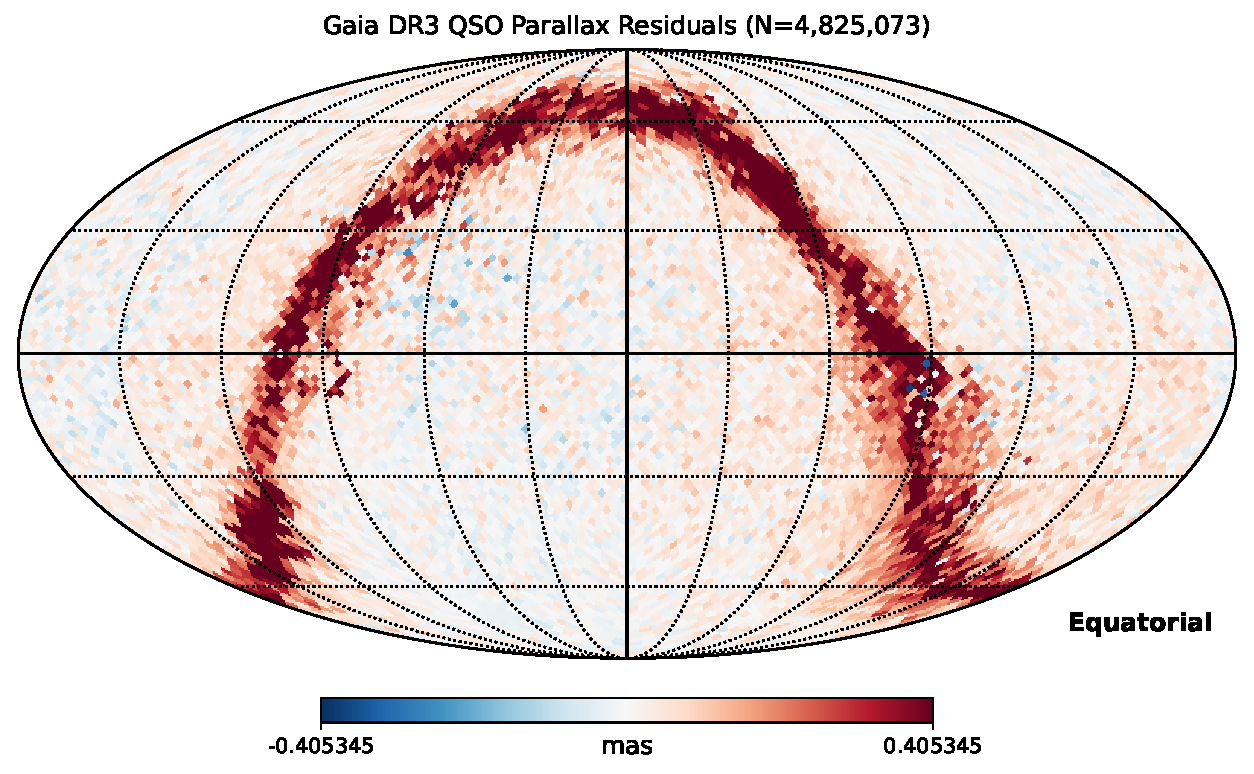
\includegraphics[width=\linewidth]{map_lorenz.pdf}
\caption{\textbf{Sky-structured parallax residual in QSO reference sample.} NSIDE=32 map of per-pixel median Gaia DR3 parallax after fixed quality cuts, Lorenz curve shown in Figure 2. The figure establishes the presence of coherent large-scale structure; concentration and leverage diagnostics are reported in Tables~1 and~2.}
\label{fig:map_lorenz}
\end{figure}

\begin{figure}[htbp]
\centering
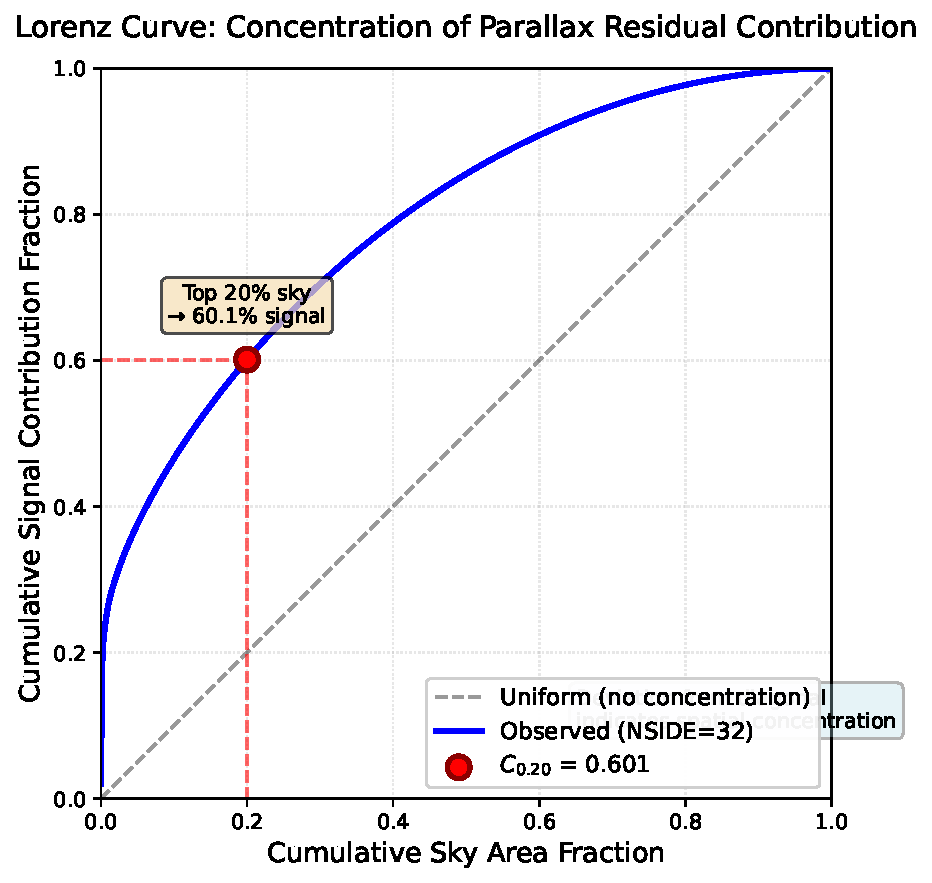
\includegraphics[width=\columnwidth]{lorenz_curve.pdf}
\caption{\textbf{Concentration diagnostic: Lorenz curve.} Top 20\% of sky carries $C_{0.20} = 0.60$ of signal, exceeding footprint null ($C_{0.20} \approx 0.34$, $p < 0.001$).}
\label{fig:lorenz}
\end{figure}

\begin{figure}[htbp]
\centering
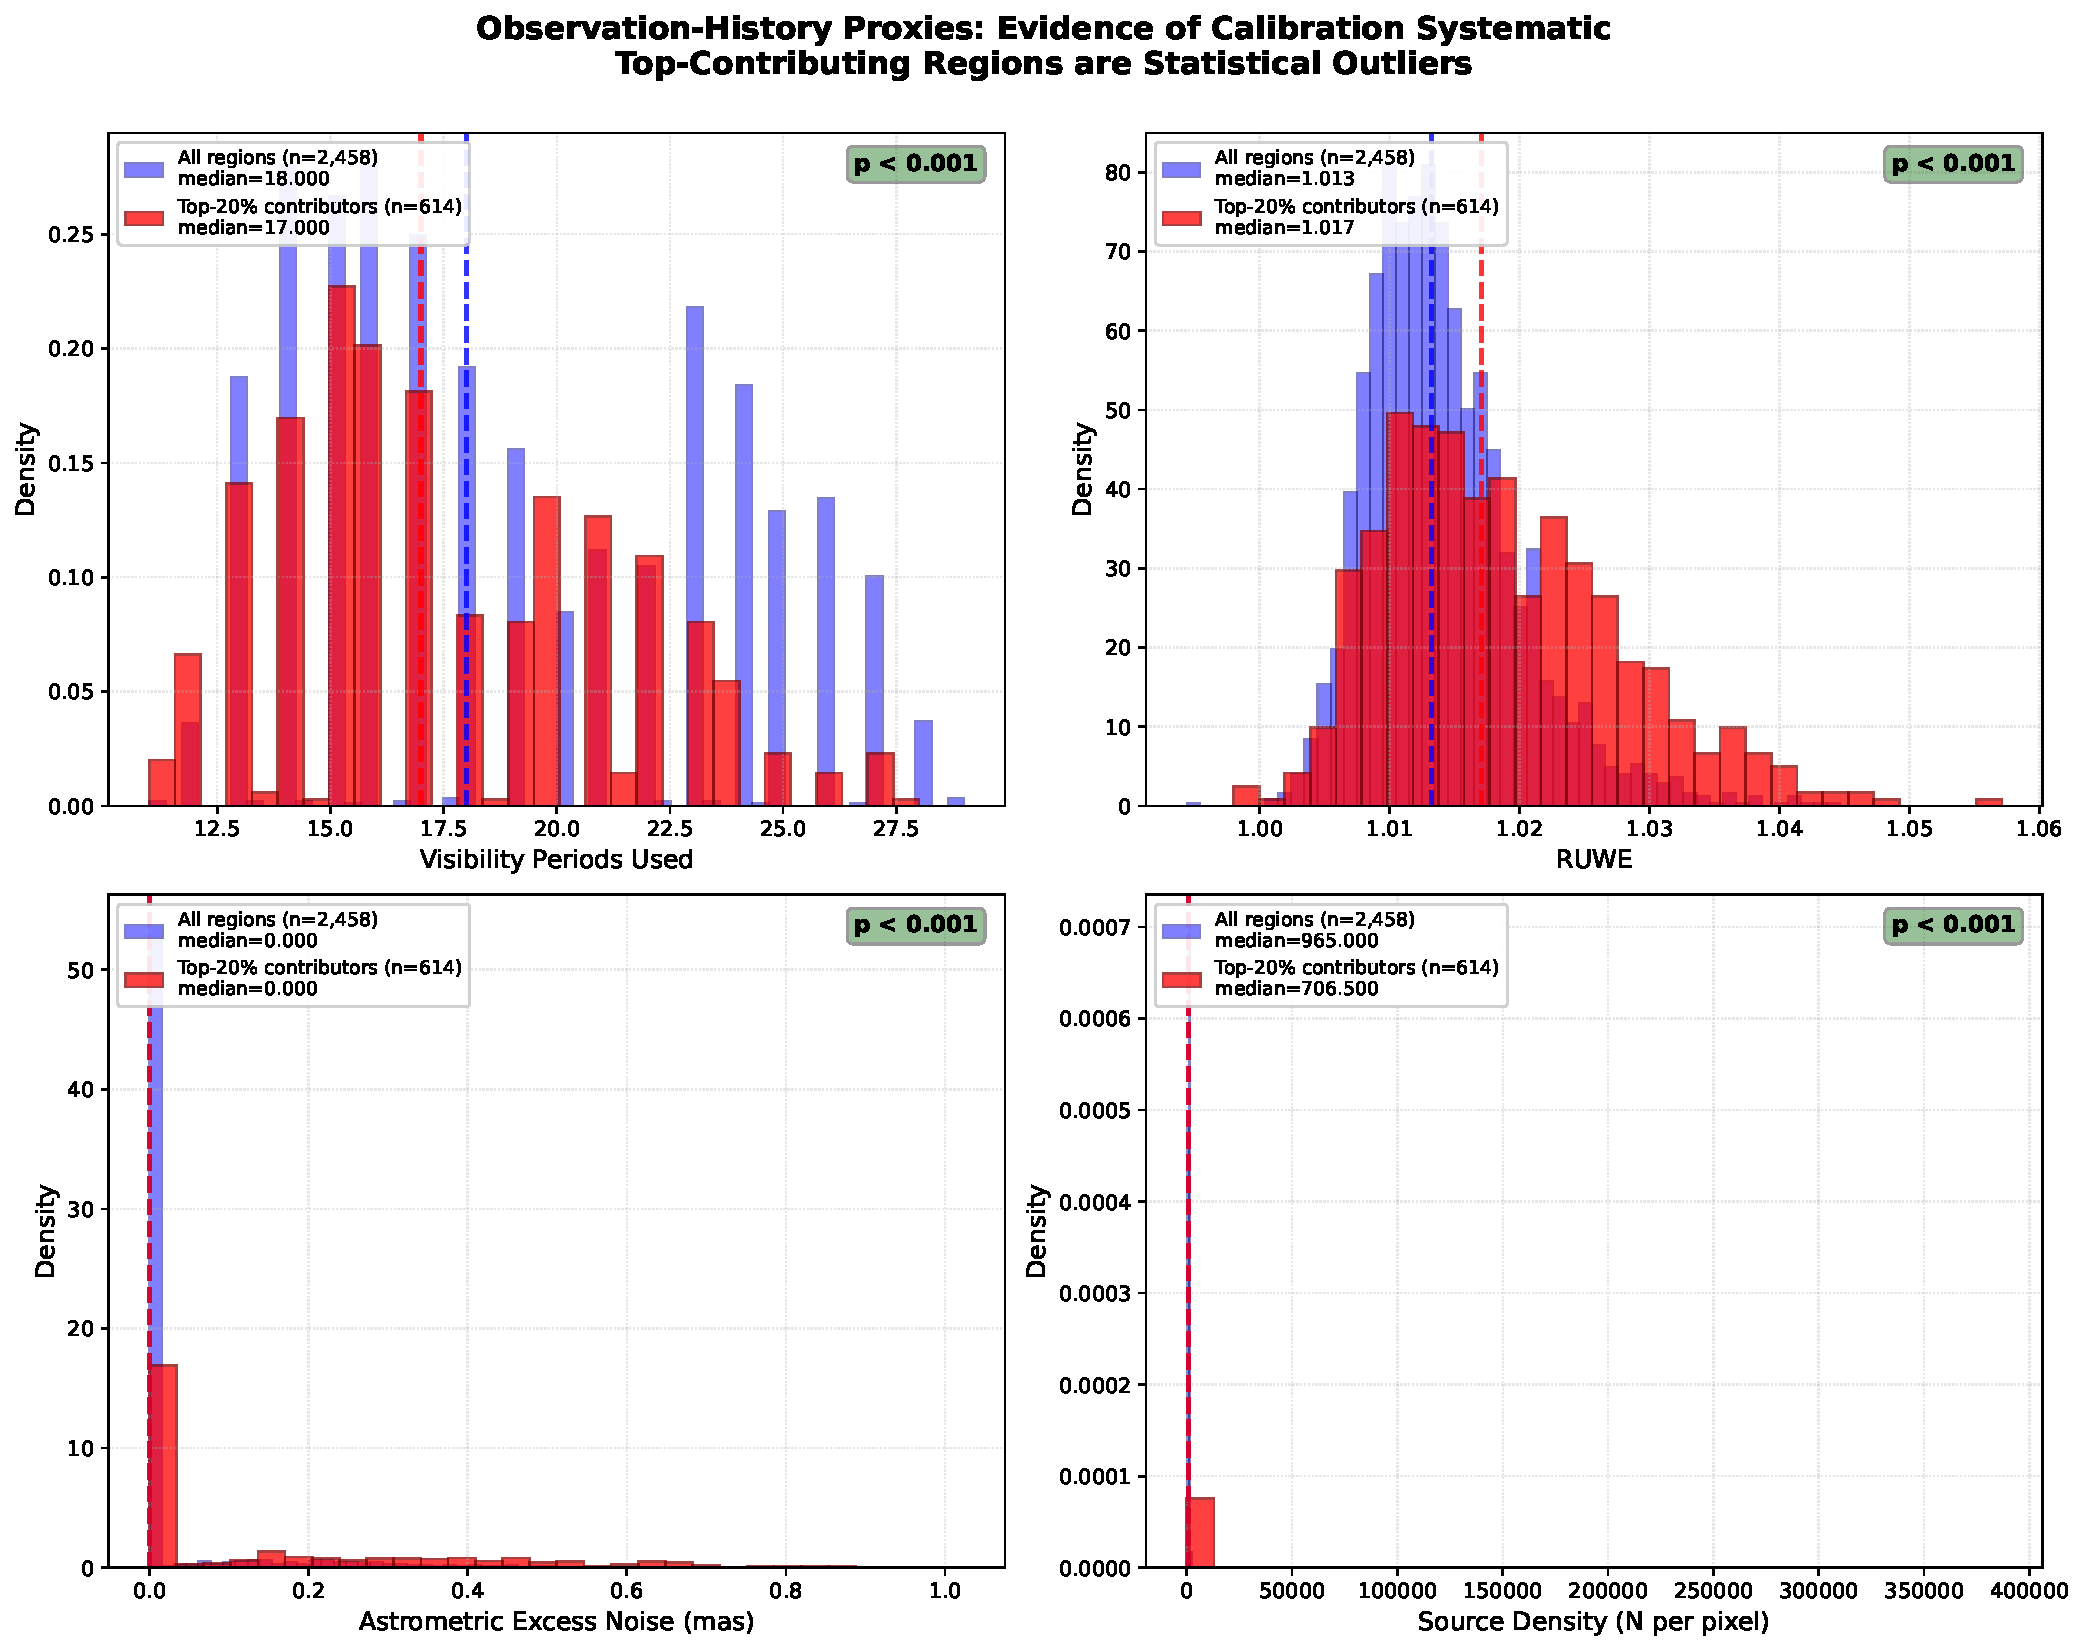
\includegraphics[width=\columnwidth]{figureS1_observation_proxies.pdf}
\caption{\textbf{Observation-history proxies.} Top-20\% contributors (red) differ significantly from all regions (blue) in observation-quality proxies (all $p < 0.001$), indicating calibration systematics.}
\label{fig:proxies}
\end{figure}
% --- END figures.tex ---

\section*{Tables}
% --- BEGIN tables.tex ---
\begin{table}
\centering
\caption{Summary of field amplitude and concentration across resolution. Baseline $S$ denotes the standard deviation of per-pixel median Gaia DR3 parallax at NSIDE=32 after fixed quality cuts. $C_{0.20}$ denotes the cumulative weighted contribution of the top 20\% sky regions at each NSIDE.}
\label{tab:summary_concentration}
\small
\begin{tabular}{@{}llc@{}}
\toprule
Metric & Value & Notes \\
\midrule
$S$ (NSIDE=32)             & 0.241 [0.223, 0.259] & Baseline$^{a}$ \\
$C_{0.20}$ (NSIDE=4)       & 0.616                & Top-20\% \\
$C_{0.20}$ (NSIDE=8)       & 0.635                & Top-20\% \\
$C_{0.20}$ (NSIDE=16)      & 0.629                & Top-20\% \\
$C_{0.20}$ (NSIDE=32)      & 0.601                & Top-20\% \\
$C_{0.20}$ (permutation null) & 0.34 [0.31, 0.37]    & 1000 perm.$^{b}$ \\
\bottomrule
\end{tabular}
\tablefoot{$^{(a)}$Std.\ dev.\ of per-pixel median parallax. $^{(b)}$Weighted $w_s = N_s|\tilde{\varpi}_s|$, at NSIDE=32.}
\end{table}


\begin{table}
\centering
\caption{Leverage under top-$K$ masking. $S$ after masking top-$K$ NSIDE=8 superpixels by contribution, relative change $\Delta S/S$, and approximate masked sky fraction (assuming ${\sim}70\%$ sky coverage at NSIDE=8 with 768 total pixels).}
\label{tab:leverage_masking}
\small
\begin{tabular}{@{}rccc@{}}
\toprule
$K$ & $S$ & $\Delta S/S$ (\%) & Masked (\%) \\
\midrule
5  & 0.235 & $-2.3$ & ${\sim}0.9$ \\
10 & 0.230 & $-4.4$ & ${\sim}1.9$ \\
20 & 0.225 & $-6.5$ & ${\sim}3.7$ \\
\bottomrule
\end{tabular}
\end{table}

% --- END tables.tex ---

% Bibliography intentionally omitted in current draft.
% \bibliographystyle{plainnat}
% \bibliography{references}

% --- BEGIN sections/data_availability.tex ---
\section*{Data Availability}

Gaia DR3 data are publicly available via the Gaia archive: \url{https://gea.esac.esa.int/archive/}

Analysis employed a locked dataset snapshot (\path{qso_merged_for_triage_analysis_ready.parquet}) containing 4,963,513 Gaia DR3 quasar candidates; quality cuts retained 4,825,073 sources (97.2\% retention). Analysis code, figure generation scripts, and processed outputs are publicly available at \url{https://github.com/blumhardt-m/gaia-qso-parallax-systematics}.

Computational environment: Python 3.13.0, pandas 2.2.0, numpy 1.24.3, healpy 1.17.0, scipy 1.11.4, matplotlib 3.8.2. All figures generated with locked quality cuts (RUWE $\leq 1.4$, visibility periods $\geq 8$) and pre-specified statistics; bootstrap resampling employed fixed seed (42) for reproducibility.

SHA256 checksums and complete provenance documentation available with analysis package.
% --- END sections/data_availability.tex ---
\clearpage
% --- BEGIN sections/references.tex ---
\section*{References}

\begin{enumerate}
\item Gaia Collaboration, Vallenari, A., Brown, A.~G.~A., et al.\ 2023, A\&A, 674, A1. \textit{Gaia Data Release 3: Summary of the content and survey properties}

\item Lindegren, L., Bastian, U., Biermann, M., et al.\ 2021a, A\&A, 649, A2. \textit{Gaia Early Data Release 3: The astrometric solution}

\item Lindegren, L., Klioner, S.~A., Hern\'andez, J., et al.\ 2021b, A\&A, 649, A4. \textit{Gaia Early Data Release 3: Parallax bias versus magnitude, colour, and position}

\item Fabricius, C., Luri, X., Arenou, F., et al.\ 2021, A\&A, 649, A5. \textit{Gaia Early Data Release 3: Catalogue validation}

\item Groenewegen, M.~A.~T.\ 2021, A\&A, 654, A20. \textit{The parallax zero-point offset from Gaia EDR3 data}

\item Ma\'iz Apell\'aniz, J., Pantaleoni Gonz\'alez, M., Barb\'a, R.~H., \& Weiler, M.\ 2021, A\&A, 649, A13. \textit{Validation of the accuracy and precision of Gaia EDR3 parallaxes with globular clusters}

\item Zinn, J.~C.\ 2021, AJ, 161, 214. \textit{Validation of the Gaia Early Data Release 3 parallax zero-point model with asteroseismology}

\item G\'orski, K.~M., Hivon, E., Banday, A.~J., et al.\ 2005, ApJ, 622, 759. \textit{HEALPix: A Framework for High-Resolution Discretization}

\item Bailer-Jones, C.~A.~L., Rybizki, J., Fouesneau, M., et al.\ 2021, AJ, 161, 147. \textit{Estimating Distances from Parallaxes}
\end{enumerate}
% --- END sections/references.tex ---
% --- BEGIN sections/appendix.tex ---
\appendix
\section{Resolution robustness and sign cancellation}
This appendix provides supporting analysis on the resolution behavior of the
concentration diagnostic and motivates the signed-aggregate definition used
throughout the main text. No additional diagnostics are introduced for inference.
The main-text statistic $C_{0.20}$, computed from $w_s = N_s|\tilde{\varpi}_s|$ with the median taken directly over sources within each superpixel, is itself of signed-aggregate (abs-after-aggregation) type at the corresponding scale; the analysis below examines the behavior of this construction under pixel refinement.

\paragraph{Resolution robustness.}
To assess sensitivity of the concentration diagnostic to angular resolution,
the signed-aggregate Top-20\% statistic was recomputed while varying the child
HEALPix resolution over
$\mathrm{NSIDE}_{\mathrm{child}} \in \{64,128,256\}$,
holding the parent grid fixed at
$\mathrm{NSIDE}_{\mathrm{parent}} = 64$.
Across this range, the signed-aggregate concentration varies modestly, from
$C_{0.20}^{\mathrm{signed}} = 0.572$ at
$\mathrm{NSIDE}_{\mathrm{child}} = 64$
to $0.540$ at $256$.
This weak dependence supports the conclusion that the detected concentration
is not an artifact of pixel-scale choice.

\paragraph{Sign cancellation in legacy definitions.}
To quantify the mechanism underlying the strong resolution dependence of
legacy concentration definitions, a sign-cancellation diagnostic is computed:
\[
\mathrm{cancel\_ratio}
= \frac{\sum_P |S_P|}{\sum_c |s_c|},
\]
where $s_c = N_c \tilde{\varpi}_c$ denotes signed child-pixel contributions and
$S_P = \sum_{c \in P} s_c$ their aggregation into parent pixels.
A value of $\mathrm{cancel\_ratio} < 1$ indicates cancellation of opposite-sign
contributions within parent pixels.
The computed $\mathrm{cancel\_ratio}$ is $1.00$ at
$\mathrm{NSIDE}_{\mathrm{child}} = 64$, decreasing to $0.64$ at $128$ and
$0.40$ at $256$.
This behavior indicates increasing within-parent sign cancellation at finer
resolution.
Consequently, legacy abs-before-sum concentration statistics exhibit strong
NSIDE dependence.
This motivates adoption of the signed-aggregate (abs-after-sum) definition as
the primary concentration metric, as it remains substantially invariant under
pixel refinement at the scales relevant to this study.

\begin{figure}[t]
\centering
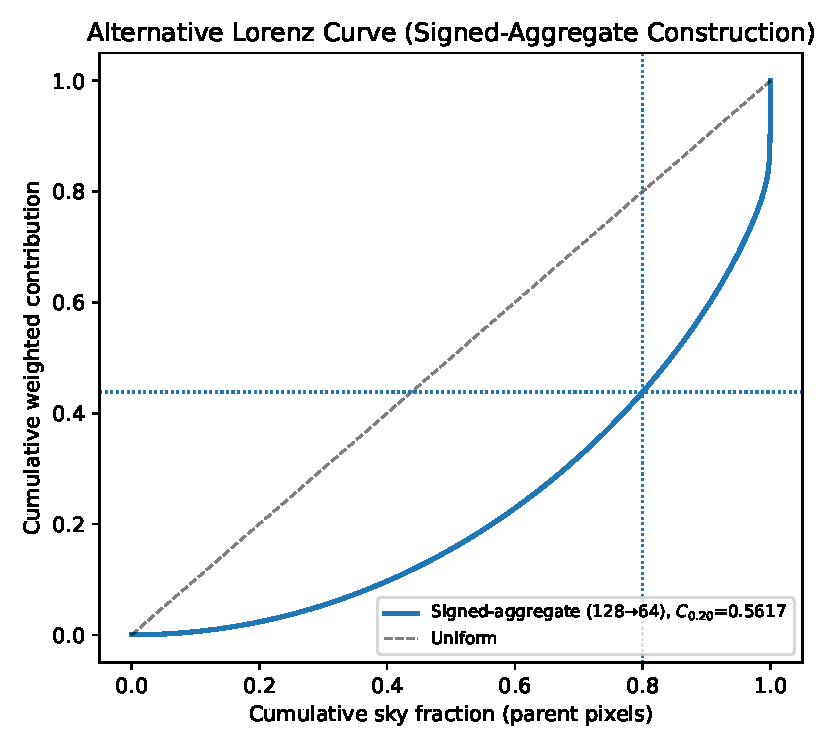
\includegraphics[width=\columnwidth]{lorenz_curve_legacy.pdf}
\caption{\textbf{Lorenz curve under the signed-aggregate construction.}
Cumulative weighted contribution computed from parent-pixel aggregates
$S_P = \sum_{c \in P} s_c$ with $\mathrm{NSIDE}_{\mathrm{child}} = 128$ and
$\mathrm{NSIDE}_{\mathrm{parent}} = 64$, yielding
$C_{0.20}^{\mathrm{signed}} = 0.562$. The absolute value is applied after
spatial aggregation, rendering the statistic substantially invariant under
pixel refinement, in contrast to the legacy abs-before-sum definition
discussed in the text.}
\label{fig:lorenz_legacy_appendix}
\end{figure}
% --- END sections/appendix.tex ---

\end{document}
